\documentclass[a4paper,12pt]{article}
\usepackage{amsmath,amssymb}
\usepackage{enumerate}
\usepackage{enumitem}
\usepackage{graphicx}
\usepackage{ wasysym }

\newcommand{\given}{\,|\,}
\newcommand{\R}{\mathbb{R}}
\newcommand{\E}{\mathbb{E}}
\newcommand{\var}{\text{var}}
\newcommand{\cov}{\text{cov}}
\newcommand{\trans}{\mathsf{T}}
\newcommand{\bx}{\mathbf{x}}
\newcommand{\by}{\mathbf{y}}
\newcommand{\bw}{\mathbf{w}}
\newcommand{\distNorm}{\mathcal{N}}
\newcommand{\bzero}{\mathbf{0}}
\newcommand{\ident}{\mathbb{I}}
\newcommand{\N}{\mathcal{N}}
\newcommand{\ep}{\varepsilon}
\newcommand{\norm}[1]{\left\lVert#1\right\rVert}

\title{CSC410 A5}
\author{Joshua Prier, }

\begin{document}
	\maketitle
	
	\begin{enumerate}
		\item 
			\begin{enumerate}
				\item \textbf{All Paths:}\\
				1,2,3,9,10,11\\
				1,2,3,9,13,14\\
				1,5,6,7,9,10,11\\
				1,5,6,7,9,13,14\\
				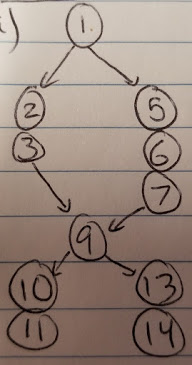
\includegraphics[scale=.5]{q1graph.jpg}
				\item 
					\begin{tabular}{|c|c|c|}
						\hline
						\multicolumn{3}{|c|}{Infeasible Path} \\
						\hline
						Line No. & Assignment & Path Conditions \\
						\hline
						1,2,3   & $x\leftarrow X-5$ & $X+Y > 10$ \\
						  ~ & $y\leftarrow Y+5$ & ~   \\
						\hline
						9,10,11  & $x\leftarrow -(X-5)$ & $X+Y > 10$ \\
						~ & $y\leftarrow -(Y+5)$ & AND $ (X-5) + (Y+5) < 0$   \\
						\hline
					\end{tabular} ~\\\\
				This path is infeasible because of the conflicting path conditions. $10 < (X+Y) = (X-5) + (Y+5) \nless 0$.
				\item 	\begin{tabular}{|c|c|c|}
					\hline
					\multicolumn{3}{|c|}{Assertion Violation Path} \\
					\hline
					Line No. & Assignment & Path Conditions \\
					\hline
					1,5,6,7   & $x\leftarrow Y$ & $X+Y \le
					 10$ \\
					~ & $y\leftarrow X$ & ~   \\
					\hline
					9,13,14  & $x\leftarrow Y-1$ & $X+Y \le 10$ \\
					~ & $y\leftarrow X-1$ & AND $ X + Y \ge 0$   \\
					\hline
				\end{tabular} ~\\\\
			This path will cause an assertion violation in the case that $X+Y \le 2$ since the assignments from 9,13,14 subtract 2 from the sum, $(X-1) + (Y-1) = X + Y - 2$\\\\
			
			\textbf{Why the other 2 paths never cause an assertion violation:}\\
			\begin{tabular}{|c|c|c|}
				\hline
				\multicolumn{3}{|c|}{Assertion Violation Path} \\
				\hline
				Line No. & Assignment & Path Conditions \\
				\hline
				1,5,6,7   & $x\leftarrow Y$ & $X+Y \le
				10$ \\
				~ & $y\leftarrow X$ & ~   \\
				\hline
				9,10,11  & $x\leftarrow -Y$ & $X+Y \le 10$ \\
				~ & $y\leftarrow -X$ & AND $ X + Y < 0$   \\
				\hline
			\end{tabular} ~\\\\
			Since  $x\leftarrow -Y$ and $y\leftarrow -X$ and $X+Y<0$ then $(X-1) + (Y-1) = -(X+Y) > 0$
		
			\begin{tabular}{|c|c|c|}
				\hline
				\multicolumn{3}{|c|}{Assertion Violation Path} \\
				\hline
				Line No. & Assignment & Path Conditions \\
				\hline
				1,2,3   & $x\leftarrow X-5$ & $X+Y >
				10$ \\
				~ & $y\leftarrow Y+5$ & ~   \\
				\hline
				9,13,14  & $x\leftarrow (X-5)-1=X-6$ & $X+Y > 10$ \\
				~ & $y\leftarrow (Y+5)-1=Y+4$ & AND $ X + Y \ge 0$   \\
				\hline
			\end{tabular} ~\\\\
			Since $X+Y>10$ then $(X-6) + (Y+4) = X+Y-2 > 10-2 = 8$ therefore $x+y > 0$
		
			\end{enumerate}
		\item \begin{enumerate}
			\item $\square b \rightarrow b \cup o$
			\item $\square \neg o \rightarrow ((r \rightarrow \ocircle w) \wedge (w \rightarrow \ocircle r)$
			\item $\square \neg o \rightarrow r \cup (b \cup (w \cup r))$
			\item $\square (r \wedge b \wedge g) \rightarrow \ocircle w$
			\item $\square r \rightarrow r \cup \neg r$
		\end{enumerate}
		\item 
		\item 
		\item 
		\item 
		\item 
	\end{enumerate}
	
\end{document}